Los tipos de interfaces podríamos definirmos de la siguiente forma:

\subsection{Control automatizado}

Este tipo de interfaces está enfocada a poder controlar dispositivos
especializados de una manera sencilla, para ayudar a los operadores
en su labor.

Un buen ejemplo es un software llamado \emph{Hevelius}~\cite{hevelius},
el cual es una aplicación que, utilizando un sistema de control
de telescopios distribuidos, utilizando un framework de desarrollo
llamado ALMA Common Software (ACS)~\cite{acs},
permite el control de un Telescopio real o un telescopio en un ambiente
simulado.

La idea principal es poder generar un entorno simple~\ref{fig:hevelius},
para tanto astronomos aficionados como profesionales,
en el cual se representan conceptos básicos del control de telescópios,
pudiendo ser un buen acercamiento al mundo de la astronomía.

\begin{figure}[!htb]
\begin{center}
    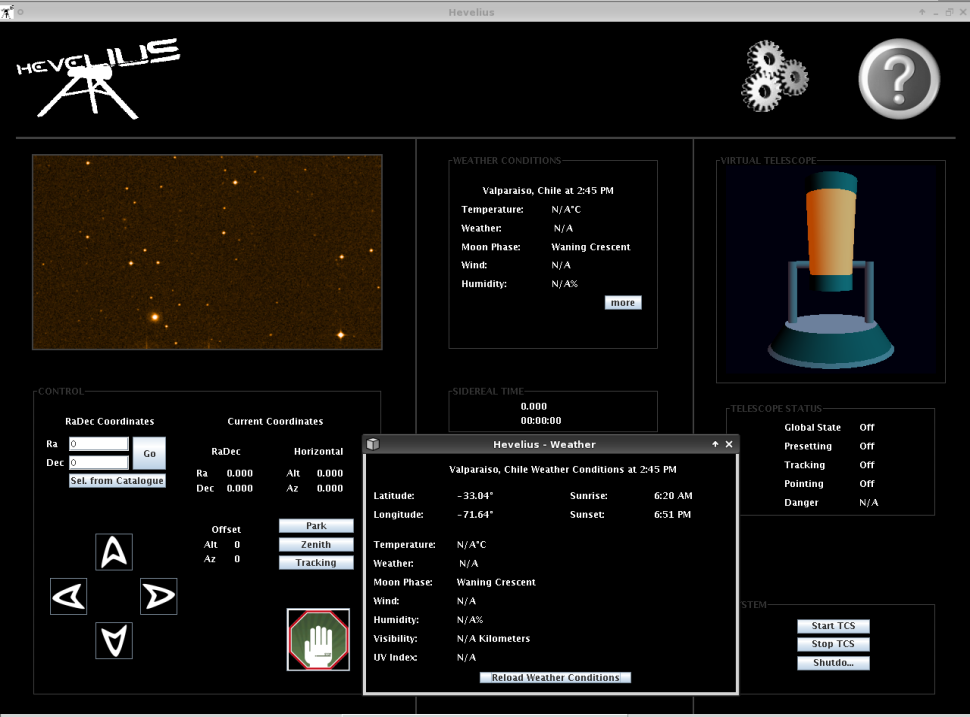
\includegraphics[width=0.4\textwidth]{img/hevelius}
    \caption{\emph{Hevelius}, ventana principal}
    \label{fig:hevelius}
\end{center}
\end{figure}

\subsection{Análisis de datos}

Otro enfoque para interfaces astronómicas, son las cuales nos permiten
poder realizar dos tareas
principales:
\begin{itemize}
    \item Obtener datos de un dispositivo o sistema (Sampling).
    \item Manipular y/o analizar los datos.
\end{itemize}

Un ejemplo que clarifica este enfoque es la herramienta llamada
\emph{Sampling System GUI (SSG)}~\cite{ssg}, la cual provee una buena
aproximación de como utilizar la API del subsistema de ACS~\cite{acs} llamado
\emph{Sampling System}~\cite{acssamp}, para poder obtener datos y
representarlos de forma gráfica~\ref{fig:ssg}, implementando una interfaz básica,
siendo su objetivo obtener la información de distintas propiedades
de dispositivos en una antena radioastronómica.

Las interfaz provee distintas opciones para realizar este proceso,
las cuales son:
\begin{itemize}
    \item Obtener datos en un periodo de tiempo,
    \item Obtener información a diferentes secuencias,
    \item Obtener información de varias propiedades en la misma ventana,
    \item Guardar datos en archivos CSV, entre otras.
\end{itemize}

\begin{figure}[!htb]
    \centering
    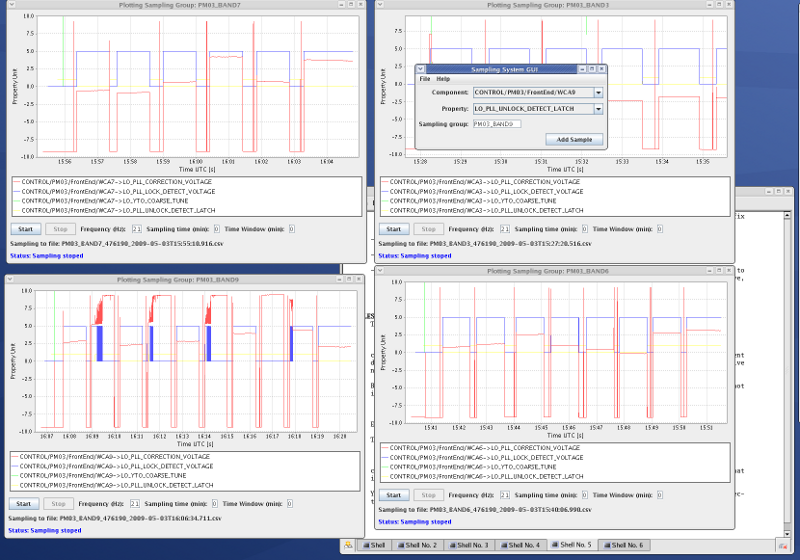
\includegraphics[width=0.4\textwidth]{img/ssg}
    \caption{\emph{Sampling System GUI}, gráficos más ventana principal}
    \label{fig:ssg}
\end{figure}

Es en esta temática, donde es muy importante realizar una elección adecuada de
dos aspectos principales, el lenguaje de programación y la biblioteca
gráfica para realizar el procedimiento de despliegue de información,
sobre todo si se trata de un sistema que recolecte información
en tiempo real.

Una investigación que aborda este problema, es el trabajo de Maureira et al~\cite{hpg}
donde presentan un estudio sobre la correcta elección entre lenguajes de programación,
(Python, C++ y Java) y algunas bibliotecas gráficas, en las cuales se definen variados
temas importantes, como por ejemplo, la simplicidad del código para poder mantenerlo,
y la cantidad de elementos que nos favorecen el trabajo a la hora de poder desarrollar
una interfaz gráfica.

\subsection{Configuraciones de sistemas}

En grandes proyectos, con una gran cantidad de variables y sistemas, que se relacionan
unos con otras, una simple accion o accidente puede provocar una cadena de reacciones
debido a la naturaleza del sistema.

Por ejemplo, si un cable de red que conecta dos computadores de pronto se corta,
todas las aplicaciones que utilizan dicha conexión fallarán, lo que provocará
que otras aplicaciones también fallen, y así sucesivamente.

¿Que problema más profundo puede ocacionar esto?
de que todos los errores de las aplicaciones y/o dispositivos pueden crear
una gran confusión al momento de buscar el problema.

Aquí una interfaz gráfica~\ref{fig:acg} llamada Alarms Configuration GUI (ACG)~\cite{acg},
la cual se basa en manipular todas las señales y configuraciones del ACS Alarm System (AS)~\cite{as},
que está a cargo de definir y reportar todas las fallas de un sistema que utilice
el framework ACS como base.

La idea de esta interfaz además es poder realizar todo este mecanismo de configuraciones,
mediante variados archivos XML, los cuales poseen la característica primordial de ser
validados mediante archivos XSD.

\begin{figure}[!htb]
    \centering
    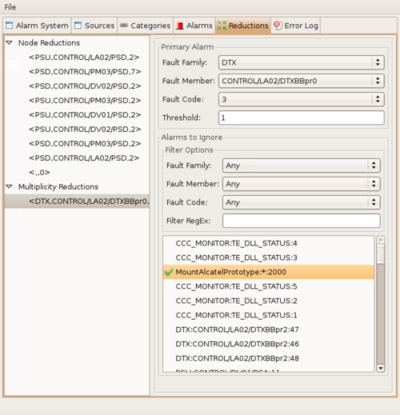
\includegraphics[width=0.4\textwidth]{img/acg}
    \caption{\emph{Alarms Configuration GUI}, ventana de propiedades}
    \label{fig:acg}
\end{figure}

\subsection{Observatorios virtuales y planetarios}

El concepto de un observatorio virtual tiene relación a un conjunto de archivos
con datos astronómicos, interactivos y que utilizan distintas
herramientas de software, en este caso, interfaces gráficas, las cuales
mediante una conexión directa con los servidores donde se encuentra
la información, pueden generar un ambiente real de trabajo,
el cual puede ser utilizado por científicos en distintos lugares del mundo.

En palabras simples, podriamos decir que un observatorio virtual es un conjunto
de centros de datos, los cuales son colecciones de datos astronómicos,
los que están apoyados por herramientas de software para realizar
cálculo científico.

La idea detrás de las interfaces gráficas consiste,
en poder automatizar distintos procesos astronómicos,
como cálculos de coordenadas, aplicar filtros, búsqueda
de datos, recuperaciónde información, etc.

%Un planetario es un lugar dedicado a la presentación de espectáculos astronómicos y en el cual es posible observar recreaciones del cielo nocturno de diversos lugares de la Tierra y en diferentes momentos del año. Normalmente un planetario consta de una pantalla de proyección en forma de cúpula y un proyector móvil capaz de proyectar las posiciones de estrellas y planetas.
%
%Algunos programas de ordenador permiten simular la posición en el cielo de las estrellas y planetas. Entre los más conocidos se encuentran los programas de código libre: Celestia, Stellarium y NightShade; no-libre pero igualmente gratuito Winstars; y de pago Starry Night.

\subsubsection{KStars}
% 1.
% KStars is a graphical desktop planetarium for KDE. It depicts an accurate simulation of the night sky, including stars, constellations, star clusters, nebulae, galaxies, all planets, the Sun, the Moon, comets and asteroids. You can see the sky as it appears from any location on Earth, on any date.
% 
% The user interface is highly intuitive and flexible. The display can be panned and zoomed with the mouse, and you can easily identify objects and track their motion across the sky. KStars includes many powerful features, yet the interface is clean and simple and fun to use.
% 
% 
% 2.
% Description
% KStars is a Desktop Planetarium for KDE. It provides an accurate graphical simulation of the night sky, from any location on Earth, at any date and time. The display includes upto 100 million stars, 13,000 deep-sky objects,all 8 planets, the Sun and Moon, and thousands of comets and asteroids.
% 
% Features
% 
% Catalogs:
%     Default catalog consisting of stars to magnitude 8
%     Extra catalogs consisting of 100 million stars to magnitude 16
%     Downloadable catalogs including Messier Images, Abell Planetary Nebulae
% Corrections for precession, nutation and atmospheric refraction
% Tools for retrieval of data from Online Databases
% Scriptable actions using D-Bus
% Integration with INDI provides support for a wide range of instruments
% Features for Educators and Students:
%     Adjustable simulation speed in order to view phenomena that happen over long timescales
%     KStars Astrocalculator to access some of the internal calculations of KStars, and also to predict conjunctions etc
%     Astroinfo project to help facilitate learning with the aid of KStars
%     Internet links for further information / pictures of objects
% Features for Amateur Astronomers:
%     Observing List tool to plan observations
%     FOV Editor helps calculate field of view of equipment and display them
%     Obtain AAVSO light curves for variable stars
%     What's up tonight tool
%     Altitude vs Time tool
%     Sky Calendar tool

\begin{figure}[!htb]
    \centering
    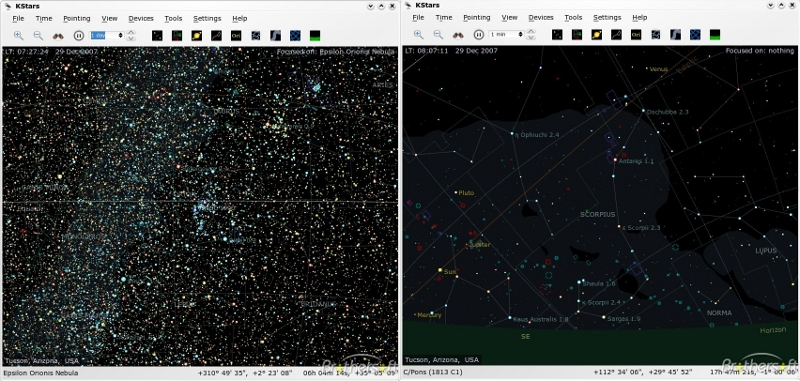
\includegraphics[width=0.5\textwidth]{img/kstars}
    \caption{\emph{KStarts}, dos vistas en la ventana principal}
    \label{fig:kstars}
\end{figure}

\subsubsection{GCX}
% 1.
% 
% Gcx is an astronomical image processing and data reduction tool, with an easy to use graphical user interface. It provides a complete set of data reduction functions for CCD photometry, with frame WCS fitting, automatic star identification, aperture photometry of target and standard stars, single-frame ensemble photometry solution finding, multi-frame color coefficient fitting, extinction coefficient fitting, and all-sky photometry; as well as general-purpose astronomical image processing functions (bias, dark, flat, frame alignment and stacking); It can function as a FITS viewer.
% 
% The program can control CCD cameras and telescopes, and implement automatic observation scripting. Cameras are controlled through a hardware-specific server, to which gcx connects through a TCP socket. It generates FITS files with comprehensive header information.
% 
% 
% 
% 2.
% The previous version of GCX , CX was written to control the newly designed cpx3m ccd camera. Once the basic camera control functions were running, it was easy to add some LX200 control functions, so that the telescope could be pointed at various objects without having to switch applications.
% 
% Having telescope control and image acquisition integrated into one program makes the following step obvious: after entering goto/get commands over several cold nights, one wants to automate the process--especially if he observes a large number of fields every night (as when doing variable star work).
% 
% The fact that the author's telescope doesn't point precisely doesn't help automation. So the ability to check/correct the pointing becomes essential. cx first got the ability to read star information from the GSC and overlay it on the images; that eases visual checks (one doesn't need maps anymore) but still is one step short of full automation.
% 
% Finally, when reliable field matching was implemented in GCX , it became possible to make the program fully automatic. In the current version, GCX can run through a list of observations completely unattended, and only stops if clouds roll in.
% 
% As it happens, field matching and image processing are also essential steps for CCD photometry. Over the time, the photometry functions of GCX have expanded continuously up to the point where they contribute the largest part of the program. It is currently possible to reduce photometric data frames in a completely automatic fashion, and perform color transformations, transformation coefficient fitting and all-sky reduction with relative ease.
% 
% Features
% 
% Image handling
% 
% Open/save 16-bit FITS image files;
% GCX uses floating-point images internally, so other FITS formats are easy to add;
% 
% Zoom/Pan images, adjust brightness/contrast/gamma in an intuitive way, appropiate for astronomical images;
% Convert FITS files to 8-bit PNM after intensity mapping;
% Show image statistics (both global and local);
% Maintain a noise model for the image across transformations; //
% Maintain bad pixel information;
% Perform ccd reductions (dark/bias/flat);
% Automatically align (register) and stack images.
% 
% Catalogs and WCS
% 
% Read field star information from GSC1/2 and Tycho2;
% Read object information from edb and native files;
% Read recipy files;
% Detect sources (stars) from images;
% Overlay objects on the image;
% Edit objects' information;
% Match image stars to catalog positions;
% Calculate world coordinates for image objects.
% 
% Camera Control
% 
% Control cameras over a TCP socket using a simple protocol;
% The control proces (cpxcntrl) presently supports the cpx3m camera. It can be easily modified to support other cameras.
% 
% Acquire images under script control;
% Set binning/windowing/integration times/temperature;
% Dark frames;
% All acquired frames are fully annotated in their FITS headers;
% Auto-generate descriptive names for files.
% 
% Telescope control
% 
% Support LX200 protocol over serial;
% Point telescope under script control;
% Point telescope by object name (if edb catalogs are installed);
% Refine pointing by comparing image star positions with catalogs;
% 
% Aperture Photometry
% 
% Do sparse field stellar photometry using fixed circular apertures for stars, annular apertures for sky estimation;
% Aperture sizes fully programmable;
% Multiple sky estimation methods;
% Uses a complex error model thorughout, that takes into account photon shot noise, read noise, noise of the callibration frames and scintillation;
% Report noise estimates for every result;
% Take photometric targets (program and standard stars) from recipy files, or directly from the image;
% Produce a comprehensive report.
% 
% Multi-Frame Reductions
% 
% Fit color transformation coefficients from multiple frames;
% Fit extinction coefficients;
% Perform all-sky reductions;
% Generate various plots for data checking;
% 
% Interfacing
% 
% Uses plain-ascii files for configuration files, reports and recipies;
% Implements import filters and an output converter to interface with tabular formats;
% Most functions available in batch mode, so the program can be made part of a script.



\begin{figure}[!htb]
    \centering
    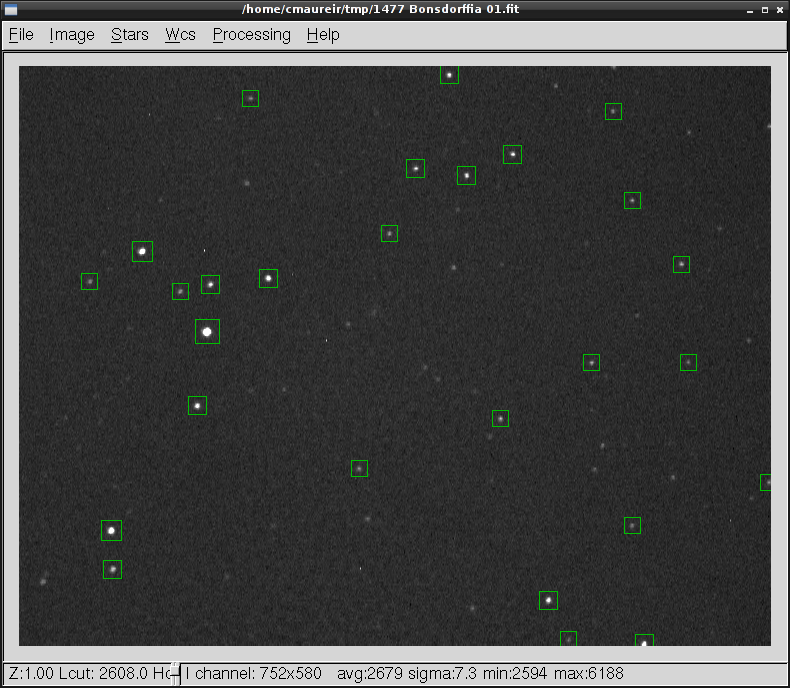
\includegraphics[width=0.5\textwidth]{img/gcx}
    \caption{\emph{GCX}, dos vistas en la ventana principal}
    \label{fig:gcx}
\end{figure}

\subsubsection{Celestia}

% Choose a point within the Local Group of galaxies, and Celestia will show you an approximation of how it would appear to your eyes were you actually there. Orbit a couple kilometers above the surface of a tiny, irregular asteroid, then head off towards Jupiter, watching it grow from a bright point of light into a looming sphere filling your field of vision.
% 
% Leave our solar system entirely and observe the sun as it fades from a brilliant disk to a bright star, disappearing almost entirely as you head off toward the Upsilon Andromeda system to orbit around its innermost giant planet.
% 
% 
% Unlike most planetarium software, Celestia doesn't confine you to the surface of the Earth. You can travel throughout the solar system, to any of over 100,000 stars, or even beyond the galaxy.
% All movement in Celestia is seamless; the exponential zoom feature lets you explore space across a huge range of scales, from galaxy clusters down to spacecraft only a few meters across. A 'point-and-goto' interface makes it simple to navigate through the universe to the object you want to visit.
% Celestia is expandable. Celestia comes with a large catalog of stars, galaxies, planets, moons, asteroids, comets, and spacecraft. If that's not enough, you can download dozens of easy to install add-ons with more objects.
% 
% 
% 
% 
% Celestia is a free real-time space simulation that lets you visually experience our universe in three dimensions.
% Celestia was the initial inspiration and creation of Mr. Chris Laurel, a Seattle, WA computer programmer who in
% 2001, decided to write a free software program to be made available to everyone on the world-wide-web that
% would place you in control of a virtual reality world of the universe. His vision and dedication gave birth to a
% program that is unlike any other space simulation program in existence. Celestia doesn't confine you to the
% surface of the Earth as do many other programs. Instead, Chris created a dynamic capability to travel throughout
% the Solar System and elsewhere in space, at any speed, at any moment of time and in any direction you choose. If
% you wish, you can fly via your own “hyperdrive” spacecraft to visit stars within the spiral arms of the Milky Way
% beyond the confines of our Sun, or leave the galaxy entirely to view the bigger universe from deep space. Chris
% also insisted this program would be scientifically accurate … a true source of dynamic astronomical graphics.


\begin{figure}[!htb]
    \centering
    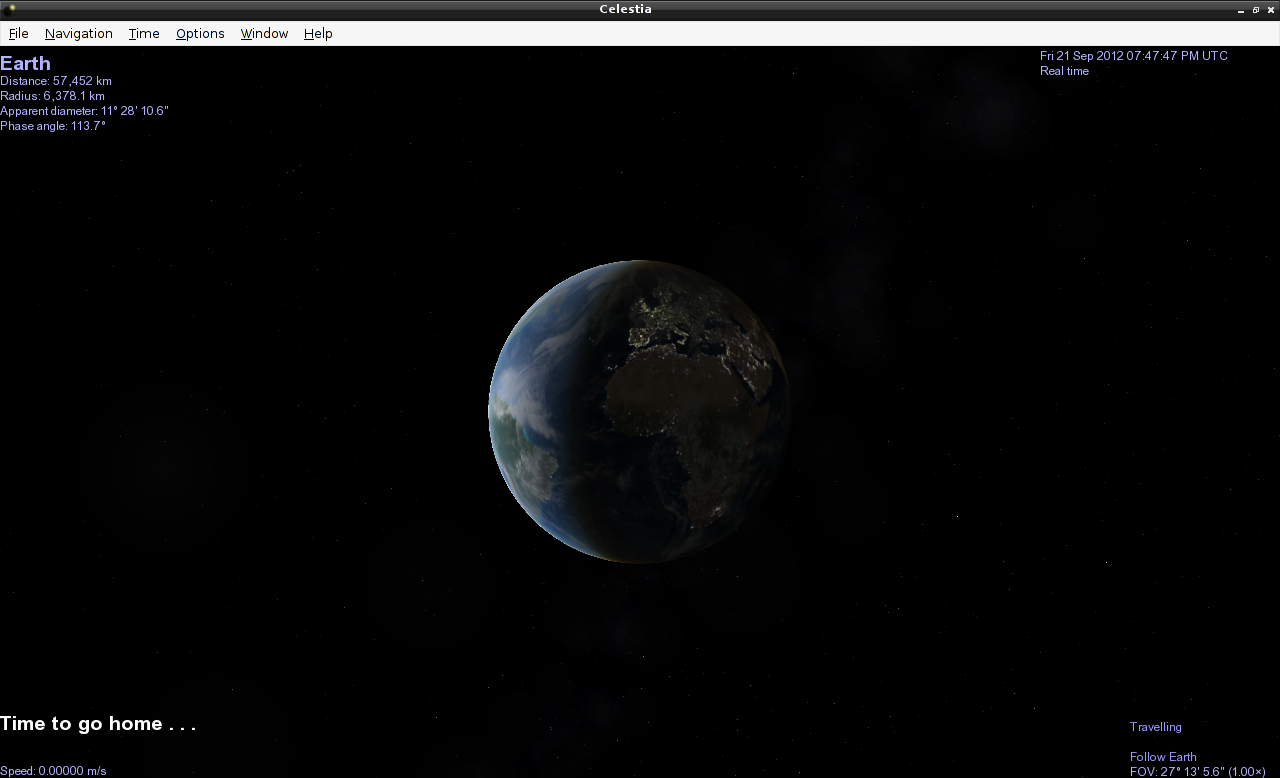
\includegraphics[width=0.5\textwidth]{img/celestia}
    \caption{\emph{Celestia}, vista de la tierra}
    \label{fig:celestia}
\end{figure}
